\section{Accumulated Muon Deflection}\label{sec:accum_defl}

As shown in Section~\ref{sec:defl_per_int}, the deflection per interaction 
is lower $\SI{1}{\degree}$. Since these deflections accumulate along the 
propagation distance, the angle between the incoming muon and the outgoing 
muon direction is simulated to study a limit on the angular reconstruction.
At first, the deflections in PROPOSAL are compared to 
the tools MUSIC and GEANT4.



\begin{figure}
    \centering
    \subcaptionbox{
        The accumulated deflection in degree is very similar in all cases.
        \label{fig:compare_MUSIC_degree}}
        {\includegraphics[width=0.48\textwidth]{figures/compare_MUSIC_degree.pdf}}
    \subcaptionbox{
        The lateral displacement builds two results in general, which depend on the scattering method. Moliére scattering leads to higher distances.
        \label{fig:compare_MUSIC_dist}}
        {\includegraphics[width=0.48\textwidth]{figures/compare_MUSIC_dist.pdf}}
    \caption{A comparison of the results of MUSIC, GEANT4 and PROPOSAL is presented for $\num{1000000}$ negative charged muons propagated with 
    $E_{\text{i}} = \SI{2}{\tera\electronvolt}$ over a distance of 
    $\SI{3}{\kilo\meter}$. A $\texttt{v\_cut} = 0.001$ is set. In PROPOSAL, 
    bremsstrahlung and photonuclear interaction are parametrized by 
    Van Ginneken (vG) and GEANT4. Detailed information are given in 
    Table~\ref{tab:compare_MUSIC}. The results for MUSIC and GEANT4 are taken from 
    \cite{comparison_MUSIC_GEANT4_2009}.}
    \label{fig:compare_MUSIC}
\end{figure}



\begin{table}
    \small
    \centering
    \caption{The survival probability $p_{\text{s}}$, the mean survived muon 
    energy $\overline{E}_{\text{f}}$, the mean scattered angle $\overline{\theta}$ 
    and the mean displacement $\overline{x}$ are presented for all cases from 
    Figure~\ref{fig:compare_MUSIC}. For all means, the standard deviation is given.
    The largest deflection and displacement result in the tool GEANT4, which has the lowest mean survived energy. The lower the energy, the larger the deflection.}
    \begin{tabular}{l|cc|cccc}
        \toprule
        & & & \multicolumn{4}{c}{PROPOSAL} \\
        &  & & \multicolumn{2}{c}{Molière} & \multicolumn{2}{c}{Highland} \\
        & MUSIC & GEANT4 & vG & GEANT4 & vG & GEANT4 \\
        \midrule
        $p_{\text{s}}\,/\,\si{\percent}$ & 77.9 & 79.3 &  \multicolumn{4}{c}{77.9}\\
        $\overline{E}_{\text{f}}\,/\,\si{\giga\electronvolt}$ & 323 & 317 & \multicolumn{4}{c}{331$\pm$178} \\
        $\overline{\theta}\,/\,\si{\degree}$ & 0.22 & 0.27 & 0.24$\pm$0.45 & 0.24$\pm$0.45 & 0.22$\pm$0.35 & 0.22$\pm$0.35   \\
        $\overline{x}\,/\,\si{\meter}$ & 2.6 & 3.3 & 2.9$\pm$2.6 & 2.9$\pm$2.6 & 2.7$\pm$1.6 & 2.7$\pm$1.7  \\
     \bottomrule
    \end{tabular}
    \label{tab:compare_MUSIC}
    \end{table}




For current analyses, it is important to study the impact of the muon 
deflection on the angular resolution to estimate a reconstruction uncertainty.
For this purpose, four different initial energies 
from $E_{\text{i}} = \SI{10}{\tera\electronvolt}$ to 
$E_{\text{i}} = \SI{10}{\peta\electronvolt}$ are used and the final 
energy is set to $E_{\text{f,\,min}} \geq \SI{10}{\giga\electronvolt}$ with 
$E_{\text{f,\,min}} < E_{\text{i}}$ for each simulation. To compare the results of 
a total of $\num{36}$ simulations, the median of the deflection distribution 
with a $\SI{95}{\percent}$ central interval is presented in 
Figure~\ref{fig:fit_median}.

\begin{equation}
    \label{eqn:fit_median}
\end{equation}


\begin{figure}
    \centering 
    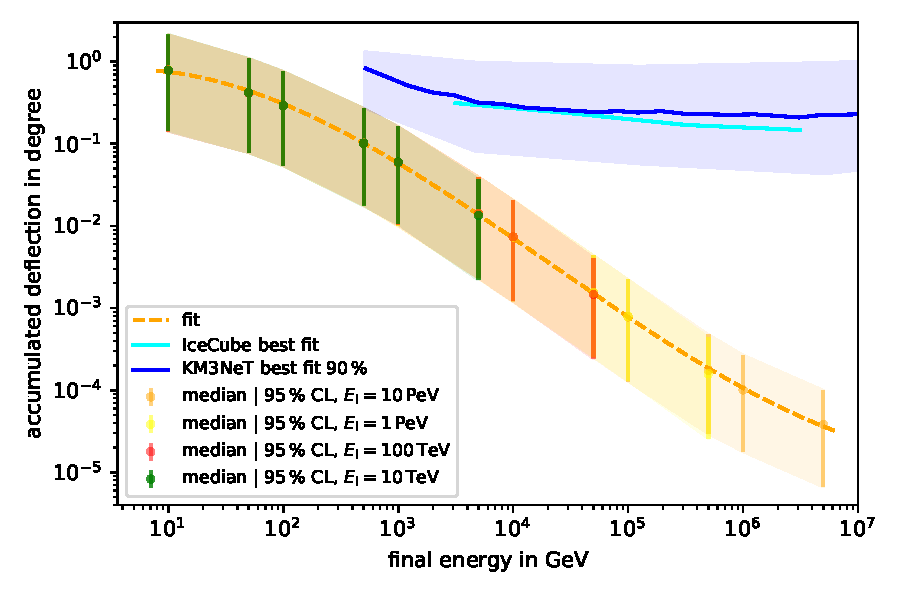
\includegraphics[width=0.8\textwidth]{figures/fit_median_defl_cut_10percent_only_poly.pdf}
    \caption{The median of the accumulated deflection with a $\SI{95}{\percent}$ 
    central interval is shown for four different initial energies $E_{\text{i}}$. 
    Each data set includes more than $\num{50000}$ events with the requirement 
    that the true final particle energy $E_{\text{f}}$ is maximum 
    $\SI{10}{\percent}$ below the set final energy $E_{\text{f,\,min}}$,   
    $E_{\text{f}} > E_{\text{f,\,min}} \cdot 0.9$. The energy cuts are $\texttt{e\_cut} = \SI{500}{\mega\electronvolt}$ and $\texttt{v\_cut} = 0.05$ and 
    Moliére scattering is chosen. 
    Since the medians overlap for different initial energies, there is no 
    strong impact of the initial energy on the median deflection. These 
    medians can be fit by a third degree polynomial in the log-space as 
    shown in Equation~\ref{eqn:fit_median}. For energies 
    $E_{\text{f}} \approx \SI{500}{\giga\electronvolt} - \SI{1}{\tera\electronvolt}$, there is a minimal influence of deflection on the angular resolution of 
    KM3NeT \cite{KM3NeT_Resolution2016}. The resolution of IceCube is not 
    impacted \cite{IceCube_Resolution2021}.}
    \label{fig:fit_median}
\end{figure}